%% DeCarvalhoDantas-ictai.tex
%%
%% Based on
%% bare_conf.tex
%% V1.3
%% 2007/01/11
%% by Michael Shell
%% See:
%% http://www.michaelshell.org/
%% for current contact information
%
\documentclass[10pt, conference, compsocconf]{IEEEtran}
% Add the compsocconf option for Computer Society conferences.
%
% If IEEEtran.cls has not been installed into the LaTeX system files,
% manually specify the path to it like:
% \documentclass[conference]{../sty/IEEEtran}

% Some very useful LaTeX packages include:
% (uncomment the ones you want to load)


% *** MISC UTILITY PACKAGES ***
%
%\usepackage{ifpdf}
% Heiko Oberdiek's ifpdf.sty is very useful if you need conditional
% compilation based on whether the output is pdf or dvi.
% usage:
% \ifpdf
%   % pdf code
% \else
%   % dvi code
% \fi
% The latest version of ifpdf.sty can be obtained from:
% http://www.ctan.org/tex-archive/macros/latex/contrib/oberdiek/
% Also, note that IEEEtran.cls V1.7 and later provides a builtin
% \ifCLASSINFOpdf conditional that works the same way.
% When switching from latex to pdflatex and vice-versa, the compiler may
% have to be run twice to clear warning/error messages.






% *** CITATION PACKAGES ***
%
%\usepackage{cite}
% cite.sty was written by Donald Arseneau
% V1.6 and later of IEEEtran pre-defines the format of the cite.sty package
% \cite{} output to follow that of IEEE. Loading the cite package will
% result in citation numbers being automatically sorted and properly
% "compressed/ranged". e.g., [1], [9], [2], [7], [5], [6] without using
% cite.sty will become [1], [2], [5]--[7], [9] using cite.sty. cite.sty's
% \cite will automatically add leading space, if needed. Use cite.sty's
% noadjust option (cite.sty V3.8 and later) if you want to turn this off.
% cite.sty is already installed on most LaTeX systems. Be sure and use
% version 4.0 (2003-05-27) and later if using hyperref.sty. cite.sty does
% not currently provide for hyperlinked citations.
% The latest version can be obtained at:
% http://www.ctan.org/tex-archive/macros/latex/contrib/cite/
% The documentation is contained in the cite.sty file itself.






% *** GRAPHICS RELATED PACKAGES ***
%
\ifCLASSINFOpdf
   \usepackage[pdftex]{graphicx}
  % declare the path(s) where your graphic files are
  % \graphicspath{{../pdf/}{../jpeg/}}
  % and their extensions so you won't have to specify these with
  % every instance of \includegraphics
  % \DeclareGraphicsExtensions{.pdf,.jpeg,.png}
\else
  % or other class option (dvipsone, dvipdf, if not using dvips). graphicx
  % will default to the driver specified in the system graphics.cfg if no
  % driver is specified.
  % \usepackage[dvips]{graphicx}
  % declare the path(s) where your graphic files are
  % \graphicspath{{../eps/}}
  % and their extensions so you won't have to specify these with
  % every instance of \includegraphics
  % \DeclareGraphicsExtensions{.eps}
\fi
% graphicx was written by David Carlisle and Sebastian Rahtz. It is
% required if you want graphics, photos, etc. graphicx.sty is already
% installed on most LaTeX systems. The latest version and documentation can
% be obtained at: 
% http://www.ctan.org/tex-archive/macros/latex/required/graphics/
% Another good source of documentation is "Using Imported Graphics in
% LaTeX2e" by Keith Reckdahl which can be found as epslatex.ps or
% epslatex.pdf at: http://www.ctan.org/tex-archive/info/
%
% latex, and pdflatex in dvi mode, support graphics in encapsulated
% postscript (.eps) format. pdflatex in pdf mode supports graphics
% in .pdf, .jpeg, .png and .mps (metapost) formats. Users should ensure
% that all non-photo figures use a vector format (.eps, .pdf, .mps) and
% not a bitmapped formats (.jpeg, .png). IEEE frowns on bitmapped formats
% which can result in "jaggedy"/blurry rendering of lines and letters as
% well as large increases in file sizes.
%
% You can find documentation about the pdfTeX application at:
% http://www.tug.org/applications/pdftex





% *** MATH PACKAGES ***
%
\usepackage[cmex10]{amsmath}
% A popular package from the American Mathematical Society that provides
% many useful and powerful commands for dealing with mathematics. If using
% it, be sure to load this package with the cmex10 option to ensure that
% only type 1 fonts will utilized at all point sizes. Without this option,
% it is possible that some math symbols, particularly those within
% footnotes, will be rendered in bitmap form which will result in a
% document that can not be IEEE Xplore compliant!
%
% Also, note that the amsmath package sets \interdisplaylinepenalty to 10000
% thus preventing page breaks from occurring within multiline equations. Use:
%\interdisplaylinepenalty=2500
% after loading amsmath to restore such page breaks as IEEEtran.cls normally
% does. amsmath.sty is already installed on most LaTeX systems. The latest
% version and documentation can be obtained at:
% http://www.ctan.org/tex-archive/macros/latex/required/amslatex/math/





% *** SPECIALIZED LIST PACKAGES ***
%
%\usepackage{algorithmic}
% algorithmic.sty was written by Peter Williams and Rogerio Brito.
% This package provides an algorithmic environment fo describing algorithms.
% You can use the algorithmic environment in-text or within a figure
% environment to provide for a floating algorithm. Do NOT use the algorithm
% floating environment provided by algorithm.sty (by the same authors) or
% algorithm2e.sty (by Christophe Fiorio) as IEEE does not use dedicated
% algorithm float types and packages that provide these will not provide
% correct IEEE style captions. The latest version and documentation of
% algorithmic.sty can be obtained at:
% http://www.ctan.org/tex-archive/macros/latex/contrib/algorithms/
% There is also a support site at:
% http://algorithms.berlios.de/index.html
% Also of interest may be the (relatively newer and more customizable)
% algorithmicx.sty package by Szasz Janos:
% http://www.ctan.org/tex-archive/macros/latex/contrib/algorithmicx/




% *** ALIGNMENT PACKAGES ***
%
%\usepackage{array}
% Frank Mittelbach's and David Carlisle's array.sty patches and improves
% the standard LaTeX2e array and tabular environments to provide better
% appearance and additional user controls. As the default LaTeX2e table
% generation code is lacking to the point of almost being broken with
% respect to the quality of the end results, all users are strongly
% advised to use an enhanced (at the very least that provided by array.sty)
% set of table tools. array.sty is already installed on most systems. The
% latest version and documentation can be obtained at:
% http://www.ctan.org/tex-archive/macros/latex/required/tools/


%\usepackage{mdwmath}
%\usepackage{mdwtab}
% Also highly recommended is Mark Wooding's extremely powerful MDW tools,
% especially mdwmath.sty and mdwtab.sty which are used to format equations
% and tables, respectively. The MDWtools set is already installed on most
% LaTeX systems. The lastest version and documentation is available at:
% http://www.ctan.org/tex-archive/macros/latex/contrib/mdwtools/


% IEEEtran contains the IEEEeqnarray family of commands that can be used to
% generate multiline equations as well as matrices, tables, etc., of high
% quality.


%\usepackage{eqparbox}
% Also of notable interest is Scott Pakin's eqparbox package for creating
% (automatically sized) equal width boxes - aka "natural width parboxes".
% Available at:
% http://www.ctan.org/tex-archive/macros/latex/contrib/eqparbox/





% *** SUBFIGURE PACKAGES ***
%\usepackage[tight,footnotesize]{subfigure}
% subfigure.sty was written by Steven Douglas Cochran. This package makes it
% easy to put subfigures in your figures. e.g., "Figure 1a and 1b". For IEEE
% work, it is a good idea to load it with the tight package option to reduce
% the amount of white space around the subfigures. subfigure.sty is already
% installed on most LaTeX systems. The latest version and documentation can
% be obtained at:
% http://www.ctan.org/tex-archive/obsolete/macros/latex/contrib/subfigure/
% subfigure.sty has been superceeded by subfig.sty.



%\usepackage[caption=false]{caption}
%\usepackage[font=footnotesize]{subfig}
% subfig.sty, also written by Steven Douglas Cochran, is the modern
% replacement for subfigure.sty. However, subfig.sty requires and
% automatically loads Axel Sommerfeldt's caption.sty which will override
% IEEEtran.cls handling of captions and this will result in nonIEEE style
% figure/table captions. To prevent this problem, be sure and preload
% caption.sty with its "caption=false" package option. This is will preserve
% IEEEtran.cls handing of captions. Version 1.3 (2005/06/28) and later 
% (recommended due to many improvements over 1.2) of subfig.sty supports
% the caption=false option directly:
%\usepackage[caption=false,font=footnotesize]{subfig}
%
% The latest version and documentation can be obtained at:
% http://www.ctan.org/tex-archive/macros/latex/contrib/subfig/
% The latest version and documentation of caption.sty can be obtained at:
% http://www.ctan.org/tex-archive/macros/latex/contrib/caption/




% *** FLOAT PACKAGES ***
%
%\usepackage{fixltx2e}
% fixltx2e, the successor to the earlier fix2col.sty, was written by
% Frank Mittelbach and David Carlisle. This package corrects a few problems
% in the LaTeX2e kernel, the most notable of which is that in current
% LaTeX2e releases, the ordering of single and double column floats is not
% guaranteed to be preserved. Thus, an unpatched LaTeX2e can allow a
% single column figure to be placed prior to an earlier double column
% figure. The latest version and documentation can be found at:
% http://www.ctan.org/tex-archive/macros/latex/base/



%\usepackage{stfloats}
% stfloats.sty was written by Sigitas Tolusis. This package gives LaTeX2e
% the ability to do double column floats at the bottom of the page as well
% as the top. (e.g., "\begin{figure*}[!b]" is not normally possible in
% LaTeX2e). It also provides a command:
%\fnbelowfloat
% to enable the placement of footnotes below bottom floats (the standard
% LaTeX2e kernel puts them above bottom floats). This is an invasive package
% which rewrites many portions of the LaTeX2e float routines. It may not work
% with other packages that modify the LaTeX2e float routines. The latest
% version and documentation can be obtained at:
% http://www.ctan.org/tex-archive/macros/latex/contrib/sttools/
% Documentation is contained in the stfloats.sty comments as well as in the
% presfull.pdf file. Do not use the stfloats baselinefloat ability as IEEE
% does not allow \baselineskip to stretch. Authors submitting work to the
% IEEE should note that IEEE rarely uses double column equations and
% that authors should try to avoid such use. Do not be tempted to use the
% cuted.sty or midfloat.sty packages (also by Sigitas Tolusis) as IEEE does
% not format its papers in such ways.





% *** PDF, URL AND HYPERLINK PACKAGES ***
%
%\usepackage{url}
% url.sty was written by Donald Arseneau. It provides better support for
% handling and breaking URLs. url.sty is already installed on most LaTeX
% systems. The latest version can be obtained at:
% http://www.ctan.org/tex-archive/macros/latex/contrib/misc/
% Read the url.sty source comments for usage information. Basically,
% \url{my_url_here}.

\usepackage{amsfonts}

% *** Do not adjust lengths that control margins, column widths, etc. ***
% *** Do not use packages that alter fonts (such as pslatex).         ***
% There should be no need to do such things with IEEEtran.cls V1.6 and later.
% (Unless specifically asked to do so by the journal or conference you plan
% to submit to, of course. )


% correct bad hyphenation here
\hyphenation{op-tical net-works semi-conduc-tor}


\begin{document}
%
% paper title
% can use linebreaks \\ within to get better formatting as desired
\title{Adaptive batch SOM for multiple dissimilarity data tables}


% author names and affiliations
% use a multiple column layout for up to two different
% affiliations

%\author{Submitted for Blind Review}

% conference papers do not typically use \thanks and this command
% is locked out in conference mode. If really needed, such as for
% the acknowledgment of grants, issue a \IEEEoverridecommandlockouts
% after \documentclass

% for over three affiliations, or if they all won't fit within the width
% of the page, use this alternative format:
% 
\author{
\IEEEauthorblockN{Anderson B. dos S. Dantas\IEEEauthorrefmark{1}, Francisco de A. T. de Carvalho\IEEEauthorrefmark{1}}

\IEEEauthorblockA{\IEEEauthorrefmark{1}Center of Informatics -- Federal University of Pernambuco (CIn/UFPE)\\
Av. Prof. Luiz Freire, s/n - Cidade Universitaria, CEP 50740-540, Recife -- PE -- Brazil\\ Email: \{absd,fatc\}@cin.ufpe.br }
}

% use for special paper notices
%\IEEEspecialpapernotice{(Invited Paper)}

% make the title area
\maketitle


\begin{abstract}
%Clustering methods for dissimilarity data are complex, but are universal and can be applied to any kind of data.
This paper introduces a clustering algorithm based on batch Self-Organizing Maps to partition objects taking into account their relational descriptions given by multiple dissimilarity matrices. 
%These matrices can be generated using different sets of variables and a fixed dissimilarity function, using a fixed set of variables and different dissimilarity functions or using different sets of variables and dissimilarity functions.
The presented approach provides a partition of the objects and a prototype for each cluster, moreover the method is able to learn relevance weights for each dissimilarity matrix by optimizing an adequacy criterion that measures the fit between clusters and the respective prototypes. These relevance weights change at each iteration and are different from one cluster to another.
%Experiments using real-world data bases are considered to show the usefulness of the method.

\end{abstract}

\begin{IEEEkeywords}
Clustering; Self-Organizing Maps; Relational data; Relevance weight; Multiple dissimilarity matrices

\end{IEEEkeywords}


% For peer review papers, you can put extra information on the cover
% page as needed:
% \ifCLASSOPTIONpeerreview
% \begin{center} \bfseries EDICS Category: 3-BBND \end{center}
% \fi
%
% For peerreview papers, this IEEEtran command inserts a page break and
% creates the second title. It will be ignored for other modes.
\IEEEpeerreviewmaketitle



\section{Introduction}
% no \IEEEPARstart
%Clustering algorithms have been used in machine learning fields including data mining, document retrieval, image segmentation and pattern recognition \cite{Jain:1999}. Clustering methods aims at organize a data set into clusters in such a way that items belonging to the same cluster have a high degree of similarity, on the other hand, items into different clusters have a high degree of dissimilarity.

Kohonen's SOM (Self-Organizing Maps) are a special type of unsupervised neural network which has clustering and visualization properties \cite{Gopalakrishnan:2008}. SOM can be considered as an algorithm that maps a high dimensional data space in a one, two or three-dimensional space. This projection enables partitioning the inputs into similar groups and has the property to preserve the topology of the data.

There are two common representations of the objects upon which clustering can be based: feature data and relational data. 
%When each object is described by a vector of quantitative or qualitative values the set of vectors describing the objects is called feature data. 
When each pair of objects is represented by a relationship, then we have relational data. The most common model of relational data is the case when we have a matrix of dissimilarity data $R = [r_{il}]$, where $r_{il}$ is the pairwise dissimilarity (often a distance) between objects $i$ and $l$.

References \cite{golli:2004} and \cite{Conan-Guez:2006} propose an adaptation of a batch SOM algorithm to dissimilarity data. Reference \cite{DeCarvalho:2011} presents a clustering algorithm that is able to partition objects taking into account simultaneously, their relational description given by multiple dissimilarity matrices.

This work proposes an approach based on batch SOM algorithm with adaptive weights to classify objects using multiple dissimilarity matrices. These matrices can be obtained using different sets of variables and a fixed dissimilarity function,
%(the final partition gives a consensus between different views describing the objects)
using a fixed set of variables and different dissimilarity functions 
%(the final partition gives the consensus between different dissimilarity functions) 
or using different sets of variables and dissimilarity functions. The influence of the different dissimilarity matrices is not equally important in the definition of the clusters in the final consensus partition \cite{Frigui:2007}. Thus, in order to obtain a meaningful partition from all dissimilarity matrices, it is necessary to learn cluster-dependent relevance weights for each dissimilarity matrix.

This paper is organized as follows. 
%Section \ref{sec:som} first describes the Self-Organizing Map algorithm as proposed by \cite{Kohonen:1990}.
Section \ref{sec:som_batch} describes a batch Self-Organizing Map algorithm for dissimilarity data proposed by \cite{golli:2004}. Section \ref{sec:adaptive_som} presents the algorithm proposed by this paper, the batch Self-Organizing Map for multiple dissimilarity data tables. To show the usefulness of this clustering algorithm, experiments with real-value data sets are considered in section \ref{sec:experiments}. Finally, Section \ref{sec:conclusion} gives the conclusions.

%%%%%%%%%%%%%%%%%%%%%%%%%%%%%%%%%%%%%%%%%%%%%%%%%%%%
% Self-Organizing Maps
%%%%%%%%%%%%%%%%%%%%%%%%%%%%%%%%%%%%%%%%%%%%%%%%%%%%
%\section{Self-Organizing Maps (SOM)}\label{sec:som}
%
%The class of methods called Self-Organizing Maps \cite{Kohonen:1990} belongs to the category of machine learning called competitive or unsupervised \cite{Murtagh:1995}. The Self-Organizing Maps algorithm involve iterative procedures to associate a finite number of objects (represented by input vectors) with a finite number of representational points, in such a way that similarity relationships between inputs are respected by these points.
%
%The architecture of SOM algorithm is composed by a set of neurons organized on a regular low-dimensional grid, generally with one, two or three dimensions called map. More formally, the map is described by a non-oriented graph ($C,\Gamma$). $C$ is a set of $m$ interconnected neurons having a discrete topology defined by $\Gamma$. The graph structure allow the definition of a distance function between two neurons in the map. For each pair of neurons (\textit{c,r}) in the map, $\delta(c,r)$ is the distance between neurons $c$ and $r$ in the graph $C$. This distance function enables a neighborhood relationship between neurons. Each neuron $c$ is represented by a p-dimensional referent vector $w_c = \{w_c^1, \dots, w_c^p\}$, where $p$ is equal to the dimension of the input vectors.
%
%The main feature of Self-Organizing Maps is the possibility of comparing clusters. Each element of the data set is affected to a cluster. Each cluster is projected to a neuron in the map. Similar elements tend to be projected in the same neuron, whereas dissimilarity grows up with the distance between two projections. The neuron with the best correspondence to a given input is updated, as well as its neighbors on the map. The region around the "winner" neuron is stretched towards the training sample presented. This procedure makes the neurons in the map to become ordered, i.e. neighboring neurons have similar referent vectors.
%
%Let $E = \{1, \dots, n\}$ the set of objects, where each object $\mathbf{x}_i = (x_{i1}, \dots, x_{ip}) (i = 1, \dots, n)$ belongs to $\mathbb{R}^p$. And, let $h_{\delta(j,l)}$ be a neighborhood function, where $\delta(j,l)$ is a fixed distance function between neurons $j$ and $l$. $h_{\delta(j,l)} = 1$ when $j = l$ and decreases to zero as $\delta(j,l)$ increases \cite{Ambroise:1996}.
%
%\subsection{SOM Algorithm}
%
%\begin{enumerate}
%\item Fix $m$, $\eta(0)$ (start learning rate), $N_{iter}$ (maximum number of iterations) and $h_{\delta(j,l)}(0)$ (start neighborhood function);
%\item Initialization: choose randomly $m$ distinct vectors as the initial prototypes $\mathbf{w}_c(0)$, $c = 1, 2, \dots, m$ and set the counter $t = 1$;
%\item Sampling: Grab a random input vector $\mathbf{x}_i(t)$;
%\item Selection: find the best Kohonen neuron (winner) $\mathbf{w}_c(t)$ in relation to minimum Euclidean distance rule:
%$$
%f(\mathbf{x}_i(t))^T = \min_{1 \leq j \leq m} \sum_{k=1}^p (x_{ik}(t) - w_{jk}(t))^2;
%$$
%\item Weight modification: for all neurons $j$ within a specified neighborhood radius of the winning neuron $\mathbf{w}_c$, adjust the weights according to the following formula:
%$$
%\mathbf{w}_j(t+1) = \mathbf{w}_j(t) + \eta (t) h_{\delta(\mathbf{w}_c, w_j)}(t)(\mathbf{x}_i(t) - \mathbf{w}_j(t));
%$$
%\item Updating: update both learning rate $\eta(t)$ and neighborhood function $h_{l,j}(t)$;
%\item Stopping criterion: if $t = N_{iter}$, stop; otherwise go to 3.
%\end{enumerate}

%%%%%%%%%%%%%%%%%
%The concept of neighborhood is taken into account through kernel functions $K$ which are positive and such that $\lim_{|x| \to \infty} K(x) = 0$ \cite{Badran:2005}. The quantity $K(\delta(c,r))$ quantifies the relative influence of the neurons on elements of the data set.

%To take advantage of the size of the neighborhood, the family of kernels $K^T$ that is parameterized by $T$ will be used: $K^T(\delta) = K (\delta / T)$. The smaller the value of $T$, the fewer the neurons that belong to the neighborhood of a given neuron $c$. The value of $T$ in the iteration $t$ is updated according to:

%\begin{equation}
%T = T_{max}\ast (\frac{T_{min}}{T_{max}})^\frac{t}{N_{iter}-1}
%\label{T}
%\end{equation}

%where$T_{min}$ and $T_{max}$ are, respectively, the final and initial values of $T$. $N_{iter}$ is the maximum number of iterations.

%Let $E = \{e_1, \dots, e_n\}$ a set of $n$ objects. The training algorithm alternates two steps. The first is the affectation step, the next performs the minimization of a cost function $J$. During the affectation step, the cost function $J$ is minimized with respect to an affectation function $f$. This function associates each observation $e_i$ to the "closest" reference vector. The Kohonen's algorithm uses the following affectation function:

%\begin{equation}
%f(e_i) = arg \min_c \parallel \mathit{e_i} - \mathbf{w}_c \parallel ^2
%\end{equation}

%And the cost function is defined by:

%\begin{equation}
%J(f, W) = \sum_{e_i \in E} \sum_{c \in C} K^T(\delta(c, f(e_i))) \parallel \mathit{e} - \mathbf{w}_c \parallel ^2.
%\label{custo_som}
%\end{equation}

%where $W$ is the set of reference vectors and $\parallel \cdot \parallel$ is a dissimilarity measure, typically the Euclidean distance. It is important to note that in this type of algorithm only one example is presented each time. the neurons of the map adjust themselves to the set of input while these are being presented. 
%
%In the minimization step the set of reference vectors $W$ are updated to minimize the cost function. The new set $W^t$ is calculated according to:
%
%\begin{equation}
%\mathit{w}_c^t = \mathit{w}_c^{t-1} - \mu^{t}K^T(\delta(c, f_t(e_i)))(\mathit{w}_c^{t-1} - e_i),
%\end{equation}
%
%where $\mu^{t}$ is the learning rate at iteration $t$.

%%%%%%%%%%%%%%%%%%%%%%%%%%%%%%%%%%%%%%%%%%%%%%%%%%%%
% SOM batch para dados de dissimilaridade
%%%%%%%%%%%%%%%%%%%%%%%%%%%%%%%%%%%%%%%%%%%%%%%%%%%%

\section{Batch Self-Organizing Map for dissimilarity data}\label{sec:som_batch}

The batch SOM algorithm for dissimilarity data (B-SOM for dissimilarity data) introduced by \cite{golli:2004} stems from the original Kohonen's SOM \cite{Badran:2005}. The main difference is on the data which are represented by a dissimilarity relationship. Let $E = \{e_1,\dots,e_n\}$ be a set of $n$ objects and a dissimilarity measure $d(e_i, e_l)$ between the objects $e_i$ and $e_l$. Each neuron $c$ is represented by a reference vector (or prototype) $g_c = e_j, \: e_j \in E$. In classical SOM each referent vector evolves in the entire input space $\mathbb{R}^p$, in this approach each neuron has a finite number of representations.

The batch training algorithm is an iterative two-step algorithm (affectation and representation steps, discussed later) in which the whole set of input (noted $E$) is presented to the map before any adjustments be achieved. %During learning the following cost function is minimized:

%\begin{equation}
%J = \sum_{i = 1}^n \sum_{r = 1}^m K^T(\delta(f(e_i),r)) d(e_i, g_r)
%\label{custo_batch}
%\end{equation}

%\noindent where $f$ is the allocation function and $f(e_i)$ stands for the neuron of the map that is associated to the object $e_i$ and $\delta(f(e_i),r)$ is the distance on the map between a neuron $r$ and the neuron that is allocated to the object $e_i$. 
The concept of neighbourhood is taken into account through kernel functions $K$ which are positive and such that $\lim_{|x| \to \infty} K(x) = 0$ \cite{Badran:2005}. Moreover, $K^T$ that is parameterized by $T$, is the neighbourhood kernel function that defines the influence region around each neuron $r$. The smaller the value of $T$, the fewer the neurons that belong to the neighbourhood of a given neuron $r$.

%This cost function is an extension of the \textit{k-means} cost function, where the Euclidean distance is replaced by a generalized distance denoted $d^T$:

%\begin{equation}
%d^T(e_i, g_{f(e_i)}) = \sum_{r=1}^m K^T(\delta(f^T(e_i), r))d(e_i, g_r)
%\label{distance}
%\end{equation}

%where
%
%\begin{equation}
%d^2(e_i, g_r) = \sum_{j=1}^p (e_{ij} - g_{rj})^2
%\label{distance2}
%\end{equation}

%\noindent is the Euclidean distance. 
%\noindent This generalized distance is a weighted sum of the euclidean distances between $e_i$ and all the prototypes of the neighbourhood of the neuron $f(e_i)$.

%The value of $T$ in the iteration $t$ is updated according to:

%\begin{equation}
%T = T_{max}\ast (\frac{T_{min}}{T_{max}})^\frac{t}{N_{iter}-1}
%\label{T}
%\end{equation}

%where$T_{min}$ and $T_{max}$ are, respectively, the final and initial values of $T$. $N_{iter}$ is the maximum number of iterations.

When T is kept fixed, the algorithm is performed iteratively in two steps: an affectation step, in which each element $e_i$ is associated to the "closest" neuron representing a referent vector followed by a representation step, in which new prototypes representing each cluster are selected.

%During affectation step, the function $f$ associates each element $e_i$ to the neuron whose referent vector is "closest" to $e_i$ and decreases the clustering criterion $J$. Each individual $e_i$ is assigned to its nearest neuron:
%
%\begin{equation}
%c = f^T(e_i) = arg \min_{1 \leq r \leq m} d^T(e_i, g_r)
%\label{f_function_batch} 
%\end{equation}

%\begin{equation}
%f(e_i) = arg \min_{c \in C} \, \sum_{l \in C}K^T(\delta(c,l)) \, d(e_i,g_l)
%\label{affectation_function} 
%\end{equation}

%During the representation step, new prototypes representing each cluster are selected. The prototype $g^*_r$ of the cluster $C_r$, which minimizes the cost function $J$ is determined by the equation:
%
%\begin{equation}
%g^*_r = arg \min_{e \in E} \sum_{i=1}^n K^T (\delta(f^T(e_i),r)) d^T(e_i, e_r)
%\label{G_batch_rossi}
%\end{equation}

%\subsection{The B-SOM Algorithm}
%
%\begin{enumerate}
%\item Initialization.\\
%Fix the number $m$ of neurons (clusters);\\
%Fix $\delta$; Fix the kernel function $K^T$;\\
%Fix the number of iterations $N_{iter}$;\\
%Fix $T_{min}$, $T_{max}$; Set $T \leftarrow T_{max}$; Set $t \leftarrow 0$;\\
%Randomly select $m$ distinct prototypes $g_c^{(0)} \in E (c = 1, \dots, m)$;\\
%Set the map $L(m, G^0)$, where $G^0 = (g_1^{(0)}, \dots, g_m^{(0)})$;\\
%Assign each object $e_i$ to the closest neuron (cluster) according to equation \ref{f_function_batch};\\
%
%\item Step 1: Representation.\\
%Set $T = T_{max}\ast (\frac{T_{min}}{T_{max}})^\frac{t}{N_{iter}-1}$;\\
%The allocation function is kept fixed;\\
%Select the prototypes $g_c^{(t)} (c = 1, \dots, m)$ according to equation \ref{G_batch_rossi};\\
%
%\item Step 2: Affectation.\\
%The prototypes $g_c^{(t)} (c = 1, \dots, m)$ are fixed. Assign each individual $e_i (i = 1, \dots, n)$ to its nearest neuron according to equation \ref{f_function_batch};\\
%
%\item Stopping criterion.
%If $T = T_{min}$ then Stop; otherwise set $t = t+1$ and go to 2 (Step 1).
%
%\end{enumerate}

%%%%%%%%%%%%%%%%%%%%%%%%%%%%%%%%%%%%%%%%%%%%%%%%
% SOM adaptive for multiple dissimilarity data
%%%%%%%%%%%%%%%%%%%%%%%%%%%%%%%%%%%%%%%%%%%%%%%%

\section{Adaptive batch Self-Organizing Map for multiple dissimilarity data tables}\label{sec:adaptive_som}

In this section we present an adaptive clustering algorithm based on both SOM for dissimilarity data \cite{golli:2004} and the clustering algorithm for multiple dissimilarity data tables \cite{DeCarvalho:2011}. The main objective of the model proposed is to map objects taking into account its relational descriptions given by multiple dissimilarity data tables.

This approach is an adaptive batch SOM algorithm (AB-SOM) that uses different adaptive weights on the dissimilarity matrices. Those weights change at each algorithm iteration and are different from one cluster to another and aims to measure the relevance of each matrix in the process of clustering. Previous works \cite{Kangas:1990}  \cite{Grozavu:2009} give adaptive versions of stochastic SOM algorithm. The computation of these vectors of weights in this algorithm is inspired from the approach used to compute a weight for each variable in each cluster in the dynamic clustering algorithm based on adaptive distances \cite{Diday:1977}.

Let $E = \{e_1,\dots,e_n\}$ be a set of $n$ objects	and let $p$ dissimilarity $n$x$n$ matrices $(\textbf{D}_1, \dots, \textbf{D}_j, \dots, \textbf{D}_p)$ where $\textbf{D}_j[i,l] = d_j(e_i,e_l)$, and $d_j(e_i,e_l)$ gives the dissimilarity between the objects $e_i$ and $e_l$ on the dissimilarity matrix $\textbf{D}_j$. Assume that the prototype $g_r$ of the cluster $C_r$ is an object of the set $E$, i.e., $g_r \in E \: \forall r = 1,\dots, c$.

The adaptive batch SOM training algorithm for multiple dissimilarity data tables introduced in this paper is an iterative three-step algorithm (affectation, representation and weighting steps) which aims to minimize the following cost function:

\begin{equation}
J = \sum_{i=1}^n \sum_{r=1}^c K^T (\delta(f^T(e_i),r)) D_{\lambda_{r}}(e_i, g_r)
\label{cost_func_adaptive}
\end{equation}

%\begin{equation}
%J = \sum_{i=1}^n \sum_{l=1}^c \exp \{- \frac{(\delta((f(e_i)),l))^2}{2T^2} \sum_{j=1}^p \lambda_{lj} d_j(e_i, g_l)
%\end{equation}

%\begin{equation}
%D_{\lambda_{r}}(e_i, g_r) = \sum_{j=1}^p \lambda_{rj} d_j(e_i, g_r)
%\end{equation}

\noindent where the kernel function $K$ is described by: $K^T(\delta) = \exp (-\frac{\delta ^2}{T^2})$ and $d_j(e_i, g_r)$ is the dissimilarity between an example $e_i \in C_r$ and the cluster prototype $g_r \in E$ parameterized by relevance weight vector $\lambda_{r} = (\lambda_{r1}, \dots, \lambda_{rj}, \dots, \lambda_{rp})$ where $\lambda_{rj}$ is the weight between the dissimilarity matrix $\textbf{D}_j$ and the cluster $C_r$. 

The relevance weight matrix $\lambda$ is composed by $c$ relevance weight vectors $\lambda_r = (\lambda_{r1},\dots,\lambda_{rj},\dots,\lambda_{rp}) (k = 1,\dots, c)$. The weight matrix changes at each iteration of the algorithm and the weight vectors are different for one cluster to another. When T is kept fixed, the algorithm alternates three steps:

\subsection*{\textbf{\textit{Step 1: Definition of the Best Prototypes}}}

In this step, the partition $P = (C_1,\dots, C_c)$ of $E$ into $c$ clusters and the relevance weight matrix $\lambda$ are fixed. The prototype $g_r \in E$ of cluster $C_r$, which minimizes the clustering criterion $J$, is computed according to:

\begin{equation}
g_r = arg \min_{e \in E} \sum_{i=1}^n K^T (\delta(f^T(e_i),r)) \sum_{j=1}^p \lambda_{rj} d_j(e_i, e)
\label{prototipo}
\end{equation}

\subsection*{\textbf{\textit{Step 2: Definition of the Best Relevance Weight Matrix}}}

In this step, the partition $P = (C_1,\dots, C_c)$ of $E$ and the vector of prototypes $g = (g_1, \dots, g_c)$ are fixed. The element $j$ of the relevance weight vector $\lambda_r = (\lambda_r1, \dots, \lambda_rp)$, which minimizes the clustering criterion $J$ under $\lambda_rj > 0$ and $\prod_{j=1}^p \lambda_rj = 1$, is calculated according to the equation:

\begin{equation}
\lambda_{rj} = \frac{\left\lbrace  \prod_{h=1}^p ( \sum_{i=1}^n K^T \delta^2(f^T(e_i), r) d_h(e_i,g_r)) \right\rbrace  ^ \frac{1}{p} }{\sum_{i=1}^n K^T \delta^2(f^T(e_i), r) d_j(e_i,g_r)}
\label{pesos}
\end{equation}

\subsection*{\textbf{\textit{Step 3: Definition of the Best Partition}}}

In this step, the vector of prototypes $g = (g_1, \dots, g_c)$ and the relevance weight matrix $\lambda$ are fixed. The cluster $C_r$, which minimize the criterion $J$, is updated according the following expression:

%\begin{eqnarray}
%r & = & f^T(e_i) \nonumber \\
%& = & arg \min_{1\leq h\leq c} \sum_{r=1}^c K^T (\delta(h,r)) \sum_{j=1}^p \lambda_{rj} d_j(e_i, g_r)
%\label{cluster}
%\end{eqnarray}

\begin{equation}
f^T(e_i) = arg \min_{1\leq h\leq c} \sum_{r=1}^c K^T (\delta(h,r)) \sum_{j=1}^p \lambda_{rj} d_j(e_i, g_r)
\label{cluster}
\end{equation}

\subsection{The AB-SOM algorithm with Relevance Weight Matrix}

\begin{enumerate}
\item Initialization.\\
Fix: the number $c$ of clusters, $\delta$, the number of iterations $N_{iter}$, $T_{min}$, $T_{max}$; Set $T \leftarrow T_{max}$; Set $t \leftarrow 0$;\\
Randomly select $c$ distinct objects $g_l \in E$;\\
Set the Relevance Weight Matrix $\lambda$ where $\lambda_l = (\lambda_{l1}, \dots, \lambda_{lp}) = (1, \dots, 1)$;\\
Set the map $M(c,\textbf{G}^0)$, where $\textbf{G}^0 = (g_1^{(0)},\dots,g_c^{(0)})$;\\
Assign each object $e_i$ the the closest prototype in order to obtain the partition $P = (C_1,\dots, C_c)$ where $C_l$ is constructed according to the equation \ref{cluster};\\

\item Step 1: definition of the best prototypes.\\
The partition $P$ and the relevance weight matrix $\lambda$ are fixed;\\
Set $T = T_{max}\ast (\frac{T_{min}}{T_{max}})^\frac{t}{N_{iter}-1}$;\\
Compute the prototype $g_l \in E$ of cluster $C_l$ according to equation \ref{prototipo}.\\

\item Step 2: definition of the best relevance weight matrix.\\
The vector of prototypes $g$ and the partition $P = (C_1,\dots, C_c)$ are fixed;\\
For each $l$, compute the component of the weight vector $\lambda_l$ according to equation \ref{pesos}.\\

\item Step 3: definition of the best partition.\\
The vector of prototypes $g$ and the relevance weight matrix $\lambda$ are fixed;\\
Assign each individual $e_i$ to its nearest neuron according to equation \ref{cluster};\\

%Construct the new partition $P' = (C'_1,\dots, C'_c)$ with the equation given by \ref{cluster} and control the convergence by:
%
%for $i=1$ to $n$ do:\\
%$e_i$ belonged to the cluster $C_m$ and belongs to the winning cluster $C'_r$\\
%if $r \neq m:\\$
%$C_r^{(t)} \leftarrow C_r^{(t)} \cup \{e_i\}$\\
%$C_m^{(t)} \leftarrow C_m^{(t)} \setminus \{e_i\}$\\

\item Stopping criterion
If $T = T_{min}$ then STOP; otherwise set $t = t+1$ and go to 2 (Step 1).

\end{enumerate}

%%%%%%%%%%%%%%%
% Experiments
%%%%%%%%%%%%%%%
\section{Experiments}\label{sec:experiments}

To illustrate the usefulness of the proposed algorithm, we used databases from the UCI Machine Learning Repository. Each attribute in the dataset is represented by a dissimilarity matrix. For the batch Self-Organizing Map for dissimilarity data algorithm, there is only one matrix available. Some measures will be considered in order to compare the results furnished by the clustering methods, they are: the corrected Rand index (CR) \cite{Hubert:1985}, the F-measure \cite{Rijsbergen:1979} and the overall error rate of classification (OERC) \cite{Breiman:1984}. In addition, the confusion matrix will be presented for each experiment. 
%The confusion matrix describes the cardinalities of all pairwise intersections between an a-priori partition and the final partition of the clustering algorithm. 
%Only non-empty clusters are shown, according to the final partition furnished by the algorithms, the matrices may have different sizes.

%The CR index assesses the degree of agreement (similarity) between an a priori partition and a partition furnished by the clustering algorithm. CR index takes its values from the interval [-1,1], in which the value 1 indicates perfect agreement between partitions, whereas values near 0 (or negatives) correspond to cluster agreement found by chance.

The variable parameters for the experiments are: topology of the map, the values of $T_{min}$ and $T_{max}$ and the total number of iterations $N_{iter}$. The topology of the map defines the maximum number of clusters that will be furnished by the algorithm. 
The values used in the experiments are the following. Topology: 2x5; $T_{min}$: 0.3; $T_{max}$: 3.0; $N_{iter}$: 500.
%Table \ref{param} shows the values of the parameters used on most of the experiments following described, 
%only in the experiment with the Wine Quality data set the parameters were different. 
Each experiment was repeated 50 times with the same values and was selected the one with the minimum adequacy criterion.

%\begin{table}[!h]
%\renewcommand{\arraystretch}{1.2}
%\begin{center}
%\caption{Parameters for the experiments}
%\label{param}
%\begin{tabular}{|c|c|}
%\hline
%Parameter & Value\\
%\hline
%Topology & 2x5\\ \hline
%$T_{min}$ & 0,3\\ \hline
%$T_{max}$ & 3,0\\ \hline
%$N_{iter}$ & 500\\ \hline
%\end{tabular}
%\end{center}
%\end{table}

\subsection{Wine data set}

This data set has results of a chemical analysis of wines grown in the same region in Italy but derived from three different cultivars, providing three classes of wine. The classes 1, 2 and 3 have, respectively 59, 71 and 48 examples. Each example is described by 13 real value attributes.

\begin{table}[!h]
\renewcommand{\arraystretch}{1.0}
\begin{center}
\caption{Wine: Confusion matrix furnished by the B-SOM algorithm}
\begin{tabular}{|c|c|c|c||c|}
\hline
Cluster/Class & 1 & 2 & 3 & Majority Class \\ \hline
0,0 & 0 & 20 & 10 & 2 \\ \hline
0,1 & 1 & 11 & 16 & 3\\ \hline
0,2 & 7 & 3 & 5 & 1\\ \hline
0,3 & 10 & 0 & 0 & 1\\ \hline
0,4 & 6 & 0 & 0 & 1\\ \hline \hline
1,0 & 0 & 25 & 2 & 2\\ \hline
1,1 & 0 & 6 & 9 & 3\\ \hline
1,2 & 5 & 5 & 6 & 3\\ \hline
1,3 & 16 & 1 & 0 & 1\\ \hline 
1,4 & 14 & 0 & 0 & 1\\ \hline
\end{tabular}
\label{wine_batch}
\end{center}
\end{table}

\begin{table}[!h]
\renewcommand{\arraystretch}{1.0}
\begin{center}
\caption{Wine: Confusion matrix furnished by the AB-SOM for multiple dissimilarity data tables}
\begin{tabular}{|c|c|c|c||c|}
\hline
Cluster/Class & 1 & 2 & 3 & Majority Class \\ \hline
0,0 & 0 & 5 & 16 & 3 \\ \hline
0,1 & 0 & 1 & 4 & 3\\ \hline
0,2 & 0 & 21 & 0 & 2\\ \hline
0,3 & 2 & 22 & 0 & 2\\ \hline
0,4 & 6 & 10 & 0 & 2\\ \hline \hline
1,0 & 0 & 0 & 15 & 3\\ \hline
1,1 & 0 & 0 & 13 & 3\\ \hline
1,2 & 0 & 9 & 0 & 2\\ \hline
1,3 & 24 & 2 & 0 & 1\\ \hline
1,4 & 27 & 1 & 0 & 1\\ \hline

\end{tabular}
\label{wine_adaptativo}
\end{center}
\end{table}

Tables \ref{wine_batch} and \ref{wine_adaptativo} give the confusion matrices furnished, respectively by the batch SOM algorithm and the adaptive approach for multiple dissimilarity tables. The last column (Majority Class) represents the number of the class with most objects in a given cluster. Observing this column it is possible to recognize regions in which objects belonging to the same a-priori class are in neighbors clusters. For example, in table \ref{wine_adaptativo}, the clusters (0,0), (0,1), (1,0) and (1,1), on the left side of the map, have more objects from class 3.
%The clusters (1,3) and (1,4) have most objects from class 1, the others have more from class 2.
%Figure \ref{fig_wine_map} shows the final map for the wine dataset furnished by the AB-SOM for multiple dissimilarity data tables. The coordinates above each cell represent the coordinates of each cluster on the map. The numbers inside the cells represent the a priori class of the majority objects.

%In figure \ref{fig_wine_map} and in table \ref{wine_adaptativo}, it is possible to recognize regions in which objects belonging to the same a-priori class are in neighbors clusters. For example, the clusters (0,0), (0,1), (1,0) and (1,1), on the left side of the map, have more objects from class 3. The clusters (1,3) and (1,4) have most objects from class 1, the others have more from class 2.

The results for CR index are 0.42 and 0.31 for, respectively, the adaptive approach for multiple dissimilarity tables and the batch SOM. For the F-measure the results are 0.52 and 0.45, respectively. And for the OERC, the results are 0.09 and 0.27, respectively. The adaptive SOM for multiple dissimilarity table performs better for the wine data set.

\begin{center}
\begin{table*}[ht]
\renewcommand{\arraystretch}{0.9}
\caption{Wine: Final relevance weight matrix}
\label{wine_pesos}
\centering
\begin{tabular}{|c|c|c|c|c|c|c|c|c|c|c|c|c|c|}
\hline
Cluster/Matrix & 1 & 2 & 3 & 4 & 5 & 6 & 7 & 8 & 9 & 10 & 11 & 12 & 13 \\ \hline
0,0 & \textbf{1.03} & 0.27 & \textbf{1.31} & \textbf{1.07} & 0.48 & 0.90 & \textbf{3.05} & 0.33 & \textbf{1.87} & \textbf{1.25} & 0.57 & \textbf{2.07} & \textbf{2.02} \\ \hline
0,1 & 0.99 & \textbf{1.05} & 0.55 & \textbf{1.09} & 0.27 & 0.69 & 0.79 & 0.52 & 0.41 & 0.92 & \textbf{1.81} & \textbf{3.60} & \textbf{8.64} \\ \hline
0,2 & \textbf{1.28} & 0.52 & 0.41 & 0.43 & \textbf{1.47} & 0.60 & \textbf{2.42} & 0.90 & \textbf{1.57} & \textbf{5.17} & 0.18 & 0.51 & \textbf{5.66} \\ \hline
0,3 & 0.69 & 0.33 & 0.93 & \textbf{2.64} & \textbf{1.32} & 0.48 & \textbf{2.29} & \textbf{1.22} & \textbf{0.45} & \textbf{2.39} & 0.36 & \textbf{4.02} & 0.62 \\ \hline
0,4 & \textbf{0.77} & \textbf{4.19} & 0.27 & 0.99 & 0.16 & \textbf{1.92} & 0.84 & \textbf{1.96} & 0.24 & \textbf{3.04} & \textbf{3.72} & \textbf{2.15} & 0.37 \\ \hline
1,0 & \textbf{1.02} & 0.37 & 0.63 & 0.89 & 0.47 & \textbf{1.68} & \textbf{2.42} & 0.25 & \textbf{2.79} & 0.45 & \textbf{1.43} & 5.12 & 0.99 \\ \hline
1,1 & 0.46 & 0.21 & 0.79 & 0.90 & \textbf{1.85} & 0.49 & \textbf{5.07} & 0.86 & 0.24 & 0.36 & \textbf{2.21} & \textbf{5.23} & \textbf{3.48} \\ \hline
1,2 & 0.42 & 0.61 & 0.51 & \textbf{1.35} & 0.16 & \textbf{2.93} & \textbf{3.12} & 0.24 & \textbf{2.27} & \textbf{2.96} & \textbf{1.33} & \textbf{1.72} & \textbf{1.01} \\ \hline
1,3 & 0.77 & 0.55 & 0.69 & 0.16 & 0.29 & \textbf{1.38} & \textbf{3.13} & \textbf{2.14} & \textbf{1.12} & \textbf{1.95} & \textbf{1.01} & \textbf{3.90} & 0.86 \\ \hline
1,4 & 0.48 & \textbf{6.01} & 0.37 & 0.33 & 0.61 & \textbf{1.64} & \textbf{1.65} & 0.94 & 0.40 & \textbf{1.50} & \textbf{1.74} & \textbf{2.78} & 0.60 \\ \hline

\end{tabular}
\end{table*}
\end{center}

%\begin{figure}[!t]
%\centering
%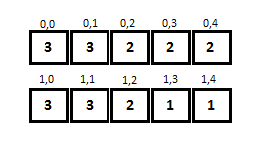
\includegraphics[width=2.5in]{Images/mapa_som.png}
%% where an .eps filename suffix will be assumed under latex, 
%% and a .pdf suffix will be assumed for pdflatex; or what has been declared
%% via \DeclareGraphicsExtensions.
%\caption{Wine: Final Map}
%\label{fig_wine_map}
%\end{figure}

Table \ref{wine_pesos} gives the final relevance weight matrix furnished by the adaptive SOM algorithm for multiple dissimilarity data tables. Values above 1 (bold in table) denote a strong influence of a given dissimilarity matrix on the cluster. For example, for the cluster (0,0) the most relevant matrix is the matrix 7 (3.05).

\subsection{Iris data set}

This data set contains 3 classes of 50 instances each, where each class refers to a type of iris plant. 
%The 3 classes are: Iris Setosa, Iris Versicolour and Iris Virginica. 
Each example is described by 4 attributes.

\begin{table}[!h]
\renewcommand{\arraystretch}{1.0}
\begin{center}
\caption{Iris: Confusion matrix from B-SOM algorithm}
\begin{tabular}{|c|c|c|c||c|}
\hline
Cluster/Class & 1 & 2 & 3 & Majority Class\\ \hline
0,0 & 0 & 1 & 15 & 3\\ \hline
0,1 & 0 & 0 & 11 & 3\\ \hline
0,2 & 0 & 0 & 9 & 3\\ \hline
0,3 & 5 & 0 & 0 & 1\\ \hline
0,4 & 32 & 0 & 0 & 1\\ \hline \hline
1,0 & 0 & 26 & 1 & 2\\ \hline
1,1 & 0 & 7 & 7 & 2/3\\ \hline
1,2 & 0 & 0 & 7 & 3\\ \hline
1,3 & 0 & 16 & 0 & 2\\ \hline
1,4 & 13 & 0 & 0 & 1\\ \hline
\end{tabular}
\label{iris_batch}
\end{center}
\end{table}

\begin{table}[!h]
\renewcommand{\arraystretch}{1.0}
\begin{center}
\caption{Iris: Confusion matrix from AB-SOM for multiple dissimilarity data tables}
\begin{tabular}{|c|c|c|c||c|}
\hline
Cluster/Class & 1 & 2 & 3 & Majority Class\\ \hline
0,0 & 13 & 0 & 0 & 1\\ \hline
0,1 & 0 & 0 & 9 & 3\\ \hline
0,2 & 0 & 17 & 0 & 2\\ \hline
0,3 & 0 & 17 & 1 & 2\\ \hline
0,4 & 0 & 4 & 14 & 3\\ \hline \hline
1,0 & 37 & 0 & 0 & 1\\ \hline
1,1 & 0 & 2 & 0 & 2\\ \hline
1,2 & 0 & 9 & 0 & 2\\ \hline
1,3 & 0 & 1 & 6 & 3\\ \hline
1,4 & 0 & 0 & 20 & 3\\ \hline

\end{tabular}
\label{iris_adaptativo}
\end{center}
\end{table}

Tables \ref{iris_batch} and \ref{iris_adaptativo} give the confusion matrices furnished, respectively by the batch SOM algorithm and the adaptive approach for multiple dissimilarity tables. In table \ref{iris_batch}, the bottom of the map has most objects from class 3 (clusters (1,0), (1,1), (1,2) and (1,3)) and in table \ref{iris_adaptativo}, class 1 is mostly present on the left side of the map (clusters (0,0) and (1,0)).

\begin{table}[!h]
\renewcommand{\arraystretch}{0.9}
\begin{center}
\caption{Iris: Final relevance weight matrix}
\begin{tabular}{|c|c|c|c|c|}
\hline
Cluster/Matrix & 1 & 2 & 3 & 4 \\ \hline
0,0 & 0.63 & 0.18 & \textbf{3.40} & \textbf{2.62} \\ \hline
0,1 & 0.80 & 0.81 & \textbf{1.45} & \textbf{1.04} \\ \hline
0,2 & 0.34 & 0.26 & \textbf{2.95} & \textbf{3.79} \\ \hline
0,3 & 0.14 & 0.29 & \textbf{10.14} & \textbf{2.26} \\ \hline
0,4 & 0.58 & 0.32 & \textbf{4.99} & \textbf{1.05} \\ \hline
1,0 & 0.25 & 0.07 & \textbf{5.06} & \textbf{11.38} \\ \hline
1,1 & \textbf{1.59} & 0.52 & 0.95 & \textbf{1.26} \\ \hline
1,2 & 0.35 & 0.50 & \textbf{1.50} & \textbf{3.73} \\ \hline
1,3 & 0.25 & \textbf{1.53} & \textbf{1.47} & \textbf{1.76} \\ \hline
1,4 & 0.51 & 0.26 & \textbf{2.59} & \textbf{2.83} \\ \hline

\end{tabular}
\label{iris_pesos}
\end{center}
\end{table}

The results for CR index are 0.54 and 0.50 for, respectively, the adaptive approach for multiple dissimilarity tables and the batch SOM. For the F-measure the results are 0.64 and 0.62, respectively. And for the OERC, the results are 0.04 and 0.06, respectively. The adaptive SOM for multiple dissimilarity table performs better for this data set.

Table \ref{iris_pesos} gives the final relevance weight matrix. In this table, the weights for the matrices 3 and 4 have greater values then the other matrices, denoting a greater influence on the objects affectation to the clusters.
%
%\subsection{Thyroid data set}
%
%Thyroid data set contains 3 classes of data representing the status of the thyroid gland. It can be at normal state, over function or under function. The three classes (1, 2 and 3) have, respectively, 150, 35 and 30 examples, each one is described by five real-value attributes.
%
%\begin{table}[!h]
%\renewcommand{\arraystretch}{1.2}
%\begin{center}
%\caption{Thyroid: Confusion matrix from B-SOM algorithm}
%\begin{tabular}{|c|c|c|c|c|c|c|c|c|c|c||c|}
%\hline
%Cluster/Class & 1 & 2 & 3 & Majority Class\\ \hline
%0,0 & 0 & 16 & 0 & 2\\ \hline
%0,1 & 10 & 0 & 3 & 1\\ \hline
%0,2 & 8 & 3 & 0 & 1\\ \hline
%0,3 & 0 & 0 & 7 & 3\\ \hline
%0,4 & 0 & 0 & 5 & 3\\ \hline \hline
%1,0 & 25 & 10 & 0 & 1\\ \hline
%1,1 & 61 & 6 & 1 & 1\\ \hline
%1,2 & 45 & 0 & 1 & 1\\ \hline
%1,3 & 1 & 0 & 4 & 3\\ \hline
%1,4 & 0 & 0 & 9 & 2\\ \hline
%
%\end{tabular}
%\label{thyroid_batch}
%\end{center}
%\end{table}
%
%\begin{table}[!h]
%\renewcommand{\arraystretch}{1.2}
%\begin{center}
%\caption{Thyroid: Confusion matrix from AB-SOM for multiple dissimilarity data tables}
%\begin{tabular}{|c|c|c|c|c|c|c|c|c|c|c||c|}
%\hline
%Cluster/Class & 1 & 2 & 3 & Majority Class\\ \hline
%0,0 & 0 & 34 & 0 & 2\\ \hline
%0,1 & 33 & 1 & 1 & 1\\ \hline
%0,2 & 22 & 0 & 0 & 1\\ \hline
%0,3 & 0 & 0 & 6 & 2\\ \hline
%0,4 & 0 & 0 & 7 & 3\\ \hline \hline
%1,0 & 29 & 0 & 0 & 1\\ \hline
%1,1 & 38 & 0 & 2 & 1\\ \hline
%1,2 & 24 & 0 & 1 & 1\\ \hline
%1,3 & 4 & 0 & 0 & 1\\ \hline
%1,4 & 0 & 0 & 13 & 3\\ \hline
%
%\end{tabular}
%\label{thyroid_adaptativo}
%\end{center}
%\end{table}
%
%Tables \ref{thyroid_batch} and \ref{thyroid_adaptativo} give the confusion matrices furnished, respectively by the batch SOM algorithm and the adaptive approach for multiple dissimilarity tables. On both tables we can see a concentration of the class 1 on the bottom left side of the map.
%
%The results for CR index are 0.37 and 0.41, respectively, for the adaptive approach for multiple dissimilarity tables and the batch SOM. For the F-measure the results are 0.52 and 0.55, respectively. And for the OERC, the results are 0.02 and 0.11, respectively. The batch SOM performs better for this data set.
%
%\begin{table}[!h]
%\renewcommand{\arraystretch}{1.2}
%\begin{center}
%\caption{Thyroid: Final relevance weight matrix}
%\begin{tabular}{|c|c|c|c|c|c|}
%\hline
%Cluster/Matrix & 1 & 2 & 3 & 4 & 5 \\ \hline
%0,0 & 0.05 & 0.15 & 0.05 & \textbf{27.94} & \textbf{85.91} \\ \hline
%0,1 & 0.37 & 0.17 & 0.20 & \textbf{19.29} & \textbf{4.14} \\ \hline
%0,2 & 0.21 & 0.29 & \textbf{4.45} & \textbf{2.61} & \textbf{1.35} \\ \hline
%0,3 & 0.14 & \textbf{2.96} & \textbf{3.01} & \textbf{1.27} & 0.61 \\ \hline
%0,4 & \textbf{5.38} & \textbf{3.21} & \textbf{1.64} & 0.86 & 0.04 \\ \hline
%1,0 & 0.28 & 0.24 & 0.35 & \textbf{9.17} & \textbf{4.59} \\ \hline
%1,1 & 0.12 & 0.24 & 0.38 & \textbf{15.75} & \textbf{5.72} \\ \hline
%1,2 & 0.14 & 0.64 & \textbf{1.53} & \textbf{27.39} & 0.26 \\ \hline
%1,3 & \textbf{1.15} & 0.91 & \textbf{4.18} & 0.24 & 0.94 \\ \hline
%1,4 & 0.91 & \textbf{9.47} & \textbf{4.83} & 0.06 & 0.38 \\ \hline
%
%\end{tabular}
%\label{thyroid_pesos}
%\end{center}
%\end{table}
%
%Table \ref{thyroid_pesos} gives the final relevance weight matrix. We can see that matrix 4 has a great relevance on most of the clusters.

%\subsection{E.coli data set}
%
%E.coli data set has information about proteins classified in eight classes. There are 336 examples described by 6 attributes, one of the attributes is the class. The distribution of the classes are following: class 1: 143 examples; class 2: 77 examples; class 3: 52 examples; class 4: 35 examples; class 5: 20 examples; class 6: 5 examples; class 7: 2 examples; class 8: 2 examples.
%
%\begin{table}[!h]
%\renewcommand{\arraystretch}{1.2}
%\begin{center}
%\caption{E.coli: Confusion matrix from B-SOM algorithm}
%\begin{tabular}{|c|c|c|c|c|c|c|c|c||c|}
%\hline
%Cluster/Class & 1 & 2 & 3 & 4 & 5 & 6 & 7 & 8 & Major Class\\ \hline
%0,0 & 47 & 0 & 0 & 0 & 5 & 1 & 0 & 0 & 1\\ \hline
%0,1 & 18 & 1 & 0 & 0 & 0 & 1 & 0 & 0 & 1\\ \hline
%0,2 & 19 & 0 & 0 & 0 & 0 & 0 & 0 & 0 & 1\\ \hline
%0,3 & 0 & 2 & 0 & 0 & 32 & 0 & 0 & 0 & 5\\ \hline
%0,4 & 0 & 25 & 1 & 1 & 24 & 1 & 0 & 0 & 2\\ \hline \hline
%1,0 & 25 & 0 & 0 & 0 & 1 & 0 & 0 & 0 & 1\\ \hline
%1,1 & 27 & 0 & 0 & 0 & 0 & 0 & 0 & 0 & 1\\ \hline
%1,2 & 6 & 0 & 0 & 1 & 0 & 13 & 4 & 8 & 6\\ \hline
%1,3 & 1 & 0 & 1 & 0 & 1 & 35 & 1 & 11 & 6\\ \hline
%1,4 & 0 & 7 & 0 & 0 & 14 & 1 & 0 & 1 & 5\\ \hline
%
%\end{tabular}
%\label{ecoli_batch}
%\end{center}
%\end{table}
%
%\begin{table}[!h]
%\renewcommand{\arraystretch}{1.2}
%\begin{center}
%\caption{E.coli: Confusion matrix from AB-SOM for multiple dissimilarity data tables}
%\begin{tabular}{|c|c|c|c|c|c|c|c|c||c|}
%\hline
%Cluster/Class & 1 & 2 & 3 & 4 & 5 & 6 & 7 & 8 & Major Class\\ \hline
%0,0 & 0 & 10 & 0 & 1 & 23 & 0 & 0 & 0 & 5\\ \hline
%0,1 & 0 & 6 & 1 & 0 & 17 & 1 & 0 & 0 & 5\\ \hline
%0,2 & 3 & 1 & 0 & 1 & 0 & 5 & 5 & 1 & 6/7\\ \hline
%0,3 & 36 & 0 & 0 & 0 & 8 & 2 & 0 & 0 & 1\\ \hline
%0,4 & 57 & 0 & 0 & 0 & 0 & 2 & 0 & 0 & 1\\ \hline \hline
%1,0 & 0 & 17 & 0 & 0 & 28 & 0 & 0 & 0 & 5\\ \hline
%1,2 & 0 & 0 & 0 & 0 & 0 & 13 & 0 & 11 & 6\\ \hline
%1,3 & 3 & 1 & 1 & 0 & 1 & 29 & 0 & 8 & 6\\ \hline
%1,4 & 44 & 0 & 0 & 0 & 0 & 0 & 0 & 0 & 1\\ \hline
%
%\end{tabular}
%\label{ecoli_adaptativo}
%\end{center}
%\end{table}
%
%Tables \ref{ecoli_batch} and \ref{ecoli_adaptativo} give the confusion matrices furnished, respectively by the batch SOM algorithm and the adaptive approach for multiple dissimilarity tables. In table \ref{ecoli_adaptativo} the cluster (1,1) has no objects, it remain empty because the cluster (1,0) has the same prototype.
%
%\begin{table}[!h]
%\renewcommand{\arraystretch}{1.2}
%\begin{center}
%\caption{Ecoli: Final relevance weight matrix}
%\begin{tabular}{|c|c|c|c|c|c|}
%\hline
%Cluster/Matrix & 1 & 2 & 3 & 4 & 5 \\ \hline
%0,0 & 0.36 & 0.50 & 0.54 & \textbf{2.55} & \textbf{3.97} \\ \hline
%0,1 & 0.49 & 0.75 & 0.55 & \textbf{2.28} & \textbf{2.16} \\ \hline
%0,2 & 0.97 & 0.89 & 0.78 & \textbf{2.09} & 0.71 \\ \hline
%0,3 & 0.87 & \textbf{1.46} & \textbf{1.13} & 0.78 & 0.89 \\ \hline
%0,4 & \textbf{1.26} & 0.90 & 0.63 & \textbf{1.21} & \textbf{1.15} \\ \hline
%1,0 & 0.50 & 0.65 & 0.64 & \textbf{2.16} & \textbf{2.20} \\ \hline
%1,1 & \textbf{1.13} & 0.75 & 0.84 & \textbf{1.45} & 0.96 \\ \hline
%1,2 & \textbf{2.44} & 0.83 & 0.26 & \textbf{1.94} & 0.98 \\ \hline
%1,3 & \textbf{2.55} & 0.53 & 0.38 & \textbf{1.54} & \textbf{1.25} \\ \hline
%1,4 & 0.48 & 0.72 & 0.46 & \textbf{2.29} & \textbf{2.70} \\ \hline
%
%\end{tabular}
%\label{ecoli_pesos}
%\end{center}
%\end{table}
%
%The results for CR index are 0.43 and 0.37, respectively, for the adaptive approach for multiple dissimilarity tables and the batch SOM. For the F-measure the results are 0.52 and 0.52, respectively. And for the OERC, the results are 0.24 and 0.24, respectively. Both algorithms perform similarly except for the CR index, in which the adaptive approach performs better.
%
%Table \ref{ecoli_pesos} gives the final relevance weight matrix. The matrix 4 has a great relevance on most clusters.

%\subsection{Wine Quality data set (wine red)}
%
%Wine quality data set consists of two datasets related to red and white variants of the Portuguese "Vinho Verde" wine \cite{Cortez:2009}. Only the red variation was considered for these experiments. There are 1599 examples, each of them is described by 11 attributes and the classification attribute. This classification is based on sensory data (median of at least 3 evaluations made by wine experts). Each expert graded the wine quality between 0 (very bad) and 10 (very excellent). In this example, the classifications of the wine red are: 3, 5, 4, 7, 6 and 8.
%
%\begin{table}[!h]
%\renewcommand{\arraystretch}{1.2}
%\begin{center}
%\caption{Wine Quality: Confusion matrix from B-SOM algorithm}
%\begin{tabular}{|c|c|c|c|c|c|c||c|}
%\hline
%Cluster/Class & 3 & 5 & 4 & 7 & 6 & 8 & Majority Class\\ \hline
%0,0 & 6 & 207 & 28 & 114 & 256 & 11 & 6\\ \hline
%0,1 & 1 & 71 & 5 & 14 & 82 & 2 & 6\\ \hline
%0,2 & 1 & 68 & 5 & 31 & 104 & 0 & 6\\ \hline
%0,3 & 2 & 149 & 9 & 23 & 135 & 3 & 5\\ \hline
%0,6 & 0 & 9 & 1 & 2 & 3 & 0 & 5\\ \hline
%0,10 & 0 & 86 & 3 & 12 & 42 & 2 & 5\\ \hline
%0,11 & 0 & 90 & 2 & 2 & 10 & 0 & 5\\ \hline
%\end{tabular}
%\label{winered_batch}
%\end{center}
%\end{table}
%
%\begin{table}[!h]
%\renewcommand{\arraystretch}{1.2}
%\begin{center}
%\caption{Wine Quality: Confusion matrix from AB-SOM for multiple dissimilarity data tables}
%\begin{tabular}{|c|c|c|c|c|c|c||c|}
%\hline
%Cluster/Class & 3 & 5 & 4 & 7 & 6 & 8 & Majority Class\\ \hline
%0,0 & 5 & 227 & 29 & 180 & 430 & 17 & 6\\ \hline
%0,3 & 4 & 426 & 23 & 9 & 177 & 1 & 5\\ \hline
%0,8 & 0 & 4 & 0 & 0 & 2 & 0 & 5\\ \hline
%0,9 & 0 & 4 & 1 & 0 & 2 & 0 & 5\\ \hline
%0,10 & 0 & 1 & 0 & 0 & 2 & 0 & 6\\ \hline
%0,11 & 1 & 19 & 0 & 9 & 20 & 0 & 6\\ \hline
%\end{tabular}
%\label{winered_adaptive}
%\end{center}
%\end{table}
%
%In this experiment, we used a 1x12 topology, and the values of $T_{min} = 0.6$, $T_{max} = 6.0$ and $N_{iter} = 500$. Tables \ref{winered_batch} and \ref{winered_adaptive} give the confusion matrices furnished, respectively by the batch SOM algorithm and the adaptive approach for multiple dissimilarity tables. In table \ref{winered_adaptive}, for example, class 5 is in the central region of the map.
%
%\begin{center}
%\begin{table*}[ht]
%\renewcommand{\arraystretch}{1.2}
%\caption{Wine Quality: Final relevance weight matrix}
%\label{winered_pesos}
%\centering
%\begin{tabular}{|c|c|c|c|c|c|c|c|c|c|c|c|}
%\hline
%Cluster/Matrix & 1 & 2 & 3 & 4 & 5 & 6 & 7 & 8 & 9 & 10 & 11 \\ \hline
%0,0 & 0.18 & 0.17 & 0.18 & 0.22 & 0.48 & 0.16 & 0.22 & \textbf{5290164.45} & 0.19 & 0.28 & 0.16 \\ \hline
%0,1 & 0.19 & 0.12 & 0.18 & 0.23 & 0.53 & 0.21 & 0.26 & \textbf{4090951.57} & 0.19 & 0.21 & 0.22 \\ \hline
%0,2 & 0.19 & 0.19 & 0.16 & 0.30 & 0.07 & 0.15 & 0.12 & \textbf{6918621.92} & 0.16 & 0.08 & \textbf{4.16} \\ \hline
%0,3 & 0.13 & 0.09 & 0.07 & 0.12 & 0.03 & 0.06 & 0.04 & \textbf{4842774.34} & 0.07 & 0.04 & \textbf{7624.27} \\ \hline
%0,4 & 0.06 & 0.04 & 0.03 & 0.06 & 0.01 & 0.03 & 0.02 & \textbf{2269275.41} & 0.03 & 0.02 & \textbf{14870482.69} \\ \hline
%0,5 & 0.07 & 0.06 & 0.05 & 0.08 & 0.02 & 0.05 & 0.04 & \textbf{6311.79} & 0.05 & 0.02 & \textbf{156727397.37} \\ \hline
%0,6 & \textbf{1.08} & \textbf{1.10} & \textbf{1.08} & \textbf{1.11} & \textbf{4.03} & 0.71 & 0.38 & \textbf{1.65} & \textbf{1.21} & 0.40 & 0.80 \\ \hline
%0,7 & 0.32 & \textbf{1.19} & 0.76 & 0.48 & \textbf{2.02} & 0.47 & 0.28 & 0.49 & \textbf{1.24} & 0.42 & \textbf{106.08} \\ \hline
%0,8 & \textbf{2.20} & 0.90 & \textbf{1.27} & 0.65 & \textbf{11.91} & \textbf{1.67} & 0.47 & 0.04 & 0.63 & 0.41 & \textbf{5.59} \\ \hline
%0,9 & \textbf{1.49} & 0.95 & 0.93 & 0.92 & \textbf{11.89} & \textbf{2.86} & \textbf{1.58} & 0.02 & 0.62 & 0.79 & \textbf{1.63} \\ \hline
%0,10 & \textbf{1.32} & \textbf{2.05} & \textbf{2.19} & 0.20 & \textbf{2.87} & 0.88 & \textbf{1.92} & 0.06 & \textbf{1.73} & \textbf{1.46} & \textbf{1.15} \\ \hline
%0,11 & \textbf{1.30} & \textbf{2.10} & \textbf{2.94} & 0.13 & \textbf{2.11} & 0.68 & \textbf{2.51} & 0.07 & \textbf{2.25} & \textbf{1.76} & \textbf{1.00} \\ \hline
%
%\end{tabular}
%\end{table*}
%\end{center}
%
%The results for CR index are 0.46 and 0.28, respectively, for the adaptive approach for multiple dissimilarity tables and the batch SOM. For the F-measure the results are 0.54 and 0.34, respectively. And for the OERC, the results are 0.44 and 0.51, respectively. The adaptive approach for multiple dissimilarity data tables performs better than the original batch SOM for this data set.
%
%Table \ref{winered_pesos} gives the final relevance weight matrix. The matrix 8 has a great relevance on most clusters.

%\begin{center}
%\begin{table}[!h]
%\renewcommand{\arraystretch}{1.2}
%\caption{Results furnished by each dataset}
%\label{final_results}
%\centering
%\begin{tabular}{|l c c c|}
%\hline
%Dataset & OERC & CR & F-Measure \\ 
%\hline
%Wine & & & \\ \hline
%B-SOM for dissimilarity data & 0.27 & 0.31 & 0.45 \\ 
%AB-SOM for multiple dissimilarity data tables & 0.09 & 0.42 & 0.52 \\ \hline
%Iris: &  &  &  \\ \hline
%B-SOM for dissimilarity data & 0.06 & 0.50 & 0.62 \\ 
%AB-SOM for multiple dissimilarity data tables & 0.04 & 0.54 & 0.64 \\ \hline
%Thyroid: &  &  &  \\ \hline
%B-SOM for dissimilarity data & 0.11 & 0.41 & 0.55 \\ 
%AB-SOM for multiple dissimilarity data tables & 0.02 & 0.37 & 0.52 \\ \hline
%E.coli: &  &  &  \\ \hline
%B-SOM for dissimilarity data & 0.24 & 0.37 & 0.52 \\ 
%AB-SOM for multiple dissimilarity data tables & 0.24 & 0.43 & 0.52 \\ \hline
%Wine red: &  &  &  \\ \hline
%B-SOM for dissimilarity data & 0.51 & 0.28 & 0.34 \\ 
%AB-SOM for multiple dissimilarity data tables & 0.44 & 0.46 & 0.54 \\ \hline
%
%\end{tabular}
%\end{table}
%\end{center}

% An example of a floating figure using the graphicx package.
% Note that \label must occur AFTER (or within) \caption.
% For figures, \caption should occur after the \includegraphics.
% Note that IEEEtran v1.7 and later has special internal code that
% is designed to preserve the operation of \label within \caption
% even when the captionsoff option is in effect. However, because
% of issues like this, it may be the safest practice to put all your
% \label just after \caption rather than within \caption{}.
%
% Reminder: the "draftcls" or "draftclsnofoot", not "draft", class
% option should be used if it is desired that figures are to be
% displayed while in draft mode.
%
%\begin{figure}[!t]
%\centering
%\includegraphics[width=2.5in]{myfigure}
% where an .eps filename suffix will be assumed under latex, 
% and a .pdf suffix will be assumed for pdflatex; or what has been declared
% via \DeclareGraphicsExtensions.
%\caption{Simulation Results}
%\label{fig_sim}
%\end{figure}

% Note that IEEE typically puts floats only at the top, even when this
% results in a large percentage of a column being occupied by floats.


% An example of a double column floating figure using two subfigures.
% (The subfig.sty package must be loaded for this to work.)
% The subfigure \label commands are set within each subfloat command, the
% \label for the overall figure must come after \caption.
% \hfil must be used as a separator to get equal spacing.
% The subfigure.sty package works much the same way, except \subfigure is
% used instead of \subfloat.
%
%\begin{figure*}[!t]
%\centerline{\subfloat[Case I]\includegraphics[width=2.5in]{subfigcase1}%
%\label{fig_first_case}}
%\hfil
%\subfloat[Case II]{\includegraphics[width=2.5in]{subfigcase2}%
%\label{fig_second_case}}}
%\caption{Simulation results}
%\label{fig_sim}
%\end{figure*}
%
% Note that often IEEE papers with subfigures do not employ subfigure
% captions (using the optional argument to \subfloat), but instead will
% reference/describe all of them (a), (b), etc., within the main caption.


% An example of a floating table. Note that, for IEEE style tables, the 
% \caption command should come BEFORE the table. Table text will default to
% \footnotesize as IEEE normally uses this smaller font for tables.
% The \label must come after \caption as always.
%
%\begin{table}[!t]
%% increase table row spacing, adjust to taste
%\renewcommand{\arraystretch}{1.3}
% if using array.sty, it might be a good idea to tweak the value of
% \extrarowheight as needed to properly center the text within the cells
%\caption{An Example of a Table}
%\label{table_example}
%\centering
%% Some packages, such as MDW tools, offer better commands for making tables
%% than the plain LaTeX2e tabular which is used here.
%\begin{tabular}{|c||c|}
%\hline
%One & Two\\
%\hline
%Three & Four\\
%\hline
%\end{tabular}
%\end{table}


% Note that IEEE does not put floats in the very first column - or typically
% anywhere on the first page for that matter. Also, in-text middle ("here")
% positioning is not used. Most IEEE journals/conferences use top floats
% exclusively. Note that, LaTeX2e, unlike IEEE journals/conferences, places
% footnotes above bottom floats. This can be corrected via the \fnbelowfloat
% command of the stfloats package.

\section{Conclusion}\label{sec:conclusion}
%The conclusion goes here. this is more of the conclusion
This paper introduced a clustering algorithm based on Self-Organizing Maps that is able to partition objects taking into account their relational descriptions given by multiple dissimilarity matrices. 
%These matrices could have been generated using different sets of variables and dissimilarity functions. 

This algorithm is an adaptive batch SOM approach for multiple dissimilarity tables. The algorithm starts from an initial partition and alternates three steps until a stop criterion is reached. 
%In the first step, the algorithm gives the solution for the best prototype of each cluster, in the second step it is determined the solution for the best relevance weight matrix. In the last step, the algorithm gives the solution of the best partition. 
These iterative steps intend to optimize an adequacy criterion that measures the fit between the partition and their prototypes. The relevance weights change at each iteration and are different from one cluster to another. 

The usefulness of this algorithm was illustrated by an experimental evaluation using real-value data sets extracted from the UCI Machine Learning Repository.
%The algorithm proposed performed better than the original batch algorithm on most of the datasets.

% conference papers do not normally have an appendix


% use section* for acknowledgement
\section*{Acknowledgment}
The authors thank the Brazilian agencies CNPq and FACEPE for their financial support.

%Acknowledgements to be added to camera ready version upon acceptance.


% trigger a \newpage just before the given reference
% number - used to balance the columns on the last page
% adjust value as needed - may need to be readjusted if
% the document is modified later
%\IEEEtriggeratref{8}
% The "triggered" command can be changed if desired:
%\IEEEtriggercmd{\enlargethispage{-5in}}

% references section

% can use a bibliography generated by BibTeX as a .bbl file
% BibTeX documentation can be easily obtained at:
% http://www.ctan.org/tex-archive/biblio/bibtex/contrib/doc/
% The IEEEtran BibTeX style support page is at:
% http://www.michaelshell.org/tex/ieeetran/bibtex/
%\nocite{*} % displays all references, cited or not
\bibliographystyle{IEEEtran}
\bibliography{DeCarvalhoDantas-ictai}
% argument is your BibTeX string definitions and bibliography database(s)
%\bibliography{IEEEabrv,../bib/paper}
%
% <OR> manually copy in the resultant .bbl file
% set second argument of \begin to the number of references
% (used to reserve space for the reference number labels box)
%\begin{thebibliography}{1}

%\bibitem{IEEEhowto:kopka}
%H.~Kopka and P.~W. Daly, \emph{A Guide to \LaTeX}, 3rd~ed.\hskip 1em plus
%  0.5em minus 0.4em\relax Harlow, England: Addison-Wesley, 1999.

%\end{thebibliography}




% that's all folks
\end{document}


